\documentclass{article}
%\usepackage{includegraphicx}
\usepackage{sydewkrpt}
\usepackage{longtable}
\usepackage{array}
\usepackage{ragged2e}
\usepackage{amsmath}
\usepackage{amssymb}
\setcounter{secnumdepth}{5}
\setcounter{tocdepth}{5}
\DeclareMathOperator*{\argmin}{\arg\!\min}
\DeclareMathOperator*{\argmax}{\arg\!\max}
\newcolumntype{P}[1]{>{\RaggedRight\hspace{0pt}}p{#1}}

%%%%%%%%%%%%%%%%%%%%%%%%%%%%
%%%    Begin Document    %%%
%%%%%%%%%%%%%%%%%%%%%%%%%%%%
\begin{document}
\pagenumbering{roman}

\waterlootitle{SYDE 462: Spring Term Final Report}{
  Group 2: Relay \\
  Adaptive Traffic Control Framework
}{
  Alex Huras -- 20344660\\
  D. Scott Neil -- 20349210\\
  Myles Tan -- 20349217\\
  Riley Donelson -- 20342815\\
  }

\dotableofcontents

\newpage
\doublespacing
\pagenumbering{arabic}

\section{Background Information}
\setlength{\parindent}{1cm}

\newpage
\section{Engineering Design}

\subsection{Front End}

\subsubsection{Design Process}
With sufficient Design Research conducted, and functional requirements compiled, the front-end application design moved into an iterative process of defining the user interface (UI), interactions, and visual design of the app through various levels of fidelity.
The use of many design tools was employed, as best suited for each given stage of the design process. 
These tools include Adobe Photoshop and Illustrator, HTML/CSS/JavaScript, and sketching using pencil and paper to quickly illustrate low-fidelity ideas.

\paragraph{Wireframing}
\mbox{ }\\ \\
The process began with a wireframing stage, involving the quick iteration of information architecture and UI techniques, to discover optimal implementations for each of the functional requirements.
Global app navigation, page layout, modularity, and fundamental UI elements were initiated at this stage, to begin to define the design language used in the application.
This was accomplished mainly through static paper-based sketches of various screens.
This allowed for rapid generation of concepts, and movement between and through ideas. 

\begin{figure}[htbp!]
  \begin{centering}
    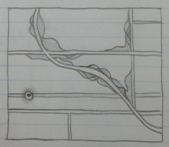
\includegraphics[scale=1]{figures/wire-1.png}
    \caption{Initial wireframe for histogram approach.}
    \label{fig:wire-1}
  \end{centering}
\end{figure}

\begin{figure}[htbp!]
  \begin{centering}
    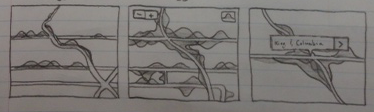
\includegraphics[scale=1]{figures/wire-2.png}
    \caption{Application wireframes showing interaction controls and pop-up menu.}
    \label{fig:wire-2}
  \end{centering}
\end{figure}

As can be seen in Figures \ref{fig:wire-1} - \ref{fig:wire-4}, various overlay techniques using both histograms and circular polygons on a map of a city were explored here in this early stage.
The histogram approach sought to model each vehicle (or small group of vehicles) on the road as a probability density function that could be moved along a road based on knowledge of traffic presence at each intersection, and speed limit data on each road.
More vehicles means more histograms, shown as translucent graphs which when overlaid, become more and more opaque, thus indicating a higher traffic density in that area.

\begin{figure}[htbp!]
  \begin{centering}
    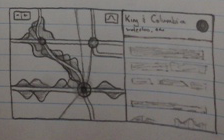
\includegraphics[scale=1]{figures/wire-4.png}
    \caption{Sketch of potential side menu for the Relay Interface application.}
    \label{fig:wire-3}
  \end{centering}
\end{figure}

Response for this concept was generally critical, as probability functions overlaid on a map were found to not be particularly easy to understand, at least not immediately at a glance.
It was evident at this stage that a simpler - more intuitive - visualization was needed for this application to be useful for both consumers and traffic engineers.\\

\begin{figure}[htbp!]
  \begin{centering}
    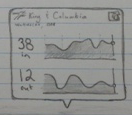
\includegraphics[scale=1]{figures/wire-5.png}
    \caption{Sketch of a detailed pop-up menu showing intersection data.}
    \label{fig:wire-4}
  \end{centering}
\end{figure}

Through exploration of the circular polygon heat-map concept, a more agreeable solution was found.
This concept modelled traffic data on a per intersection basis.
In other words, when an intersection is experiencing a high volume of traffic, a translucent circular polygon is triggered and overlaid onto a map of the city at the longitude and latitude of the intersection.
The size of the circle is positively correlated to the volume of traffic at the intersection.
A second degree of data is then shown through use of colour, to illustrate the performance of the intersection itself.
This gives insight into how well the intersection is moving traffic given it's high-volume state.
It was agreed upon that a well-performing high-volume intersection should receive a colour that is neutral, while a high-volume intersection with poor performance should emit a colour that indicates that something is wrong, such as orange or red.

It can also be seen in the figures that other components of the prototype application were accounted for in the wireframes.
These include interactions such as pop-up dialogues, highlighting routes and communicating intersections, as well as a side-panel for showing detailed metrics on intersection and overall city-wide traffic performance.
From this stage, the prototype moved to a mid-fidelity phase to further build out the concepts and refine the aesthetic of the application.

While not all of these early-stage concepts were used in the final product, the process of generating, critiquing, and refining multiple ideas proved valuable throughout the year.
These initial visualization concepts helped to spawn and guide future implementations, and helped attain a clear understanding of the data being presented.
The next step in the design process moved into a medium-fidelity stage, such that navigation and interaction could be explored at a deeper level.

\paragraph{Medium-Fidelity Prototyping}
Through the use of prototyping software Balsamiq, a set of interactive mockups were created to both reflect the requirements of the application, as well as ideas and lessons learned from the previous wireframing stage.
In this prototype, the main tenets for the final version of the application were created in an illustrative form, to identify key architectural components and the user's interaction within.
By doing this in a medium that does not put too much focus on the specifics of visual design, it was easier to concentrate on the core features of the application, and how they satisfy (or dissatisfy) the original requirements. 

At this stage, the concept of data layers was explored.
Given that there are many varying metrics identified as important to target users (Traffic Engineers), and that these metrics all have a spatial or location-based relevance, the idea of turning on and off layers of data visualization overlaid on a map was critical in effectively demonstrating traffic data.
Metrics such as intersection Status, and Flow through an intersection were conceptualized at this stage, with some preliminary UI put together for interacting with these layers.
A screenshot of the mockup showing a Status visualization in the Relay app is presented in Figure \ref{fig:bals-1}. \\

\begin{figure}[htbp!]
  \begin{centering}
    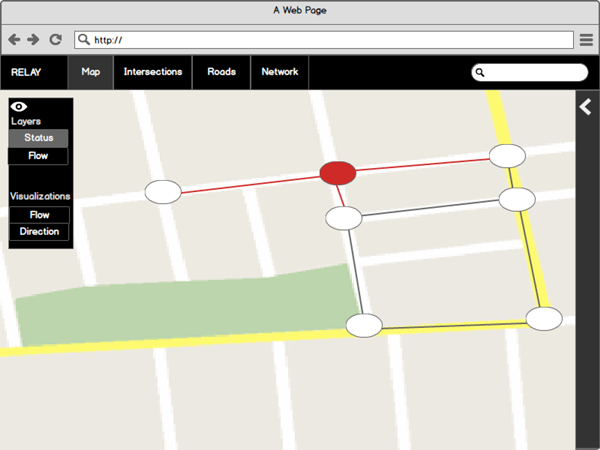
\includegraphics[scale=0.6]{figures/bals-1.png}
    \caption{Balsamiq mockup of a data layer in the Relay app.}
    \label{fig:bals-1}
  \end{centering}
\end{figure}

Additionally, as can be seen at the top of Figure \ref{fig:bals-1} the foundations for global app navigation was built out, in the form of a fixed header bar at the top of the screen.
This header serves many purposes, including branding for the app, search functionality, as well as tabbed buttons to move between contextually grouped pages.
Figure \ref{fig:bals-1} shows the active state of the Map button, while the main area of the screen contains a map with relevant data.

Further interaction was carried out at this stage, in the form of a modular popup window, referred to as the Relay info box.
This info box was designed to present deeper metrics for an intersection, and appears when an intersection on the map is clicked.
This allows users to quickly inspect any intersection of interest and monitor time-series data in the context of a specific location.
A Balsamiq mockup of the info box is presented in Figure \ref{fig:bals-2}.

\begin{figure}[htbp!]
  \begin{centering}
    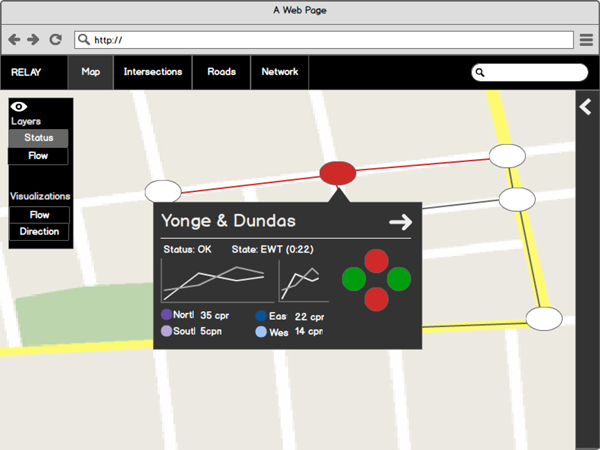
\includegraphics[scale=0.6]{figures/bals-2.png}
    \caption{Balsamiq mockup of the Relay info box.}
    \label{fig:bals-2}
  \end{centering}
\end{figure}

\paragraph{High-Fidelity Prototyping}


\subsection{Back End}

\subsection{Deep End}

\newpage
\section{Design Testing and Validation}

\subsection{Front End}

\subsection{Back End}

\subsection{Deep End}

\newpage
\section{Recommended Design Modifications}

\newpage
\section{Timeline and Project Management}

\newpage
\section{Conclusion}

\newpage
\addcontentsline{toc}{section}{References}

\bibliographystyle{IEEEtran}

\bibliography{bib}

\end{document}
